\section{Chương 2: Thực nghiệm và đánh giá}
\label{sec:evaluation}

\subsection{Câu hỏi thực nghiệm và thiết lập}
\todo{A nêu câu hỏi: correctness, ảnh hưởng minsup, dense/sparse, BitVector,
scalability và transaction length. B review tính công bằng.}
\todo{Điền CPU, RAM, OS, Julia/Java/SPMF, thread count, seed, warm-up, số lần lặp,
median/spread, timeout và phạm vi timer. Phân biệt internal read+mine với
end-to-end wall-clock; không so hai phạm vi khác nhau như một metric.}

\subsection{Dữ liệu benchmark}
\begin{table}[htbp]
\centering
\caption{Thống kê trên đúng file benchmark dùng trong thí nghiệm; các ô chờ đo.}
\label{tab:datasets}
\begin{tabular}{lrrr}
\toprule
CSDL & $n$ & $m$ & Width TB \\
\midrule
Chess & -- & -- & -- \\
Mushroom & -- & -- & -- \\
Retail & -- & -- & -- \\
T10I4D100K & -- & -- & -- \\
\bottomrule
\end{tabular}
\end{table}
Trong Bảng~\ref{tab:datasets}, $n$ là số giao dịch, $m$ là số item phân biệt và width
là số item/giao dịch. \todo{Bổ sung nguồn snapshot HF/Kaggle, version/hash, license,
preprocessing và đặc điểm dense/sparse; tính số từ file thật.}

\subsection{Đối chiếu correctness với SPMF}
\todo{B so đầy đủ itemset/support cho từng CSDL/minsup; bảng n_patterns,
missing, extra, wrong support và exact match rate. Nêu denominator, trường hợp
output rỗng và phân tích mọi sai khác. Không chỉ so tổng số pattern.}

\subsection{Runtime và output size theo minsup}
\todo{A chèn bốn đồ thị runtime (basic, BitVector, SPMF), 5--7 ngưỡng giảm dần/tập;
median + spread, đơn vị, legend, caption và tham chiếu từng hình trong lời văn.
Chèn output-size curves, giải thích bằng intersection và candidate/output growth.}

% Example only: replace path after a real run; do not insert fabricated figures.
% \begin{figure}[htbp]
% \centering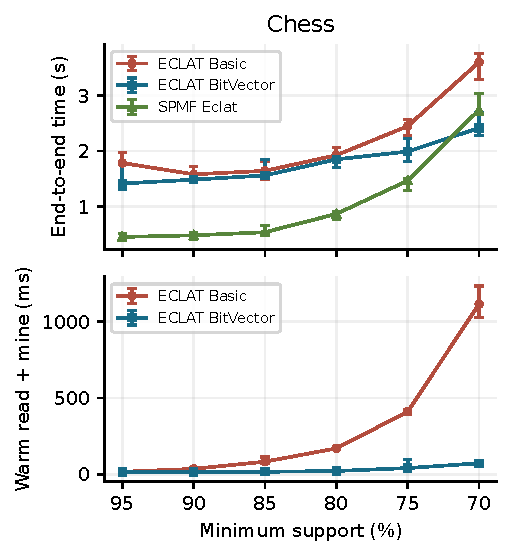
\includegraphics[width=\columnwidth]{figures/runtime-chess.pdf}
% \caption{Runtime trên Chess theo minsup, cùng phạm vi đo; TODO số lần lặp.}
% \label{fig:runtime-chess}
% \end{figure}

\subsection{Peak RAM và hiệu quả tối ưu}
\todo{A đo peak RSS basic/BitVector tại minsup trung bình của từng dataset.
Nêu công cụ OS và vòng đời process; không coi allocations là peak memory hoặc
so RSS với heap log. Bổ sung speedup và memory reduction từ số đo thật.}

\subsection{Scalability và độ dài giao dịch}
\todo{Retail: nested subsets 10/25/50/75/100\%, relative minsup cố định, tính
absolute count theo n thực. Vẽ runtime theo n, kèm output size và giới hạn sampling.}
\todo{Synthetic: n, m, seed, minsup cố định; transaction widths tăng dần; trình bày
runtime/output, mô tả generator mẫu và khác biệt với generator trong paper.}

\subsection{Thảo luận, hạn chế và tối ưu tiếp theo}
\todo{Giải thích xu hướng bằng mô tả thuật toán và complexity; nêu trường hợp
BitVector có lợi/bất lợi, JIT/JVM, I/O, warm-up, timeout/OOM và giới hạn phần cứng.}
\todo{Đề xuất ít nhất 2 hướng tối ưu cụ thể có cơ sở: ví dụ adaptive list/bitset,
buffer reuse, ordering/early-stop. Phân biệt điều đã đo với giả thuyết tương lai.}
